\documentclass[twoside,11pt]{article}

% Any additional packages needed should be included after jmlr2e.
% Note that jmlr2e.sty includes epsfig, amssymb, natbib and graphicx,
% and defines many common macros, such as 'proof' and 'example'.
%
% It also sets the bibliographystyle to plainnat; for more information on
% natbib citation styles, see the natbib documentation, a copy of which
% is archived at http://www.jmlr.org/format/natbib.pdf

\usepackage{jmlr2e}

% Definitions of handy macros can go here

\newcommand{\dataset}{{\cal D}}
\newcommand{\fracpartial}[2]{\frac{\partial #1}{\partial  #2}}

% Heading arguments are {volume}{year}{pages}{submitted}{published}{author-full-names}

\jmlrheading{(volume-tbd)}{2023}{pp-pp}{3/23}{mm/yy}{Xudong Sun, and others
}

% Short headings should be running head and authors last names

\ShortHeadings{DomainLab: A python package for domain generalization in deep learning
}{Xudong Sun, and others
}
\firstpageno{1}

\begin{document}

\title{DomainLab: A python package for domain generalization in deep learning
}

\author{\name Xudong Sun \email xudong.sun@helmholtz-muenchen.de \\
\addr Institute of AI for Health\\
Helmholtz Munich\\
Munich, Germany
\AND
\name Carsten Marr \email carsten.marr@helmholtz-muenchen.de \\
\addr Institute of AI for Health\\
Helmholtz Munich\\
Munich, Germany
}

\editor{tbd}

\maketitle

\begin{abstract}%   <- trailing '%' for backward compatibility of .sty file
\input{abstract_domainlab}
\end{abstract}

\begin{keywords}
Domain Generalization, Deep Learning, Python

\end{keywords}

\section{Summary}\label{sec:summary}
Deep learning (DL) models have been used in tackling real-world
challenges in various areas, such as computer vision and medical imaging
or computational pathology. However, while generalizing to unseen data
domains comes naturally to humans, it is still a significant obstacle
for machines. By design, most DL models assume that training and testing
distributions are well aligned, causing them to fail when this is
violated. Instead, domain generalization aims at training domain
invariant models that are robust to distribution shifts~\cite{wang2022generalizing}.

We introduce DomainLab, a Python package for domain generalization.
Compared to existing and concurrent solutions, DomainLab excels at the
extent of modularization by decoupling the various factors that
contribute to the performance of a domain generalization method: How the
domain invariant regularization loss is computed remain decoupled and
transparent to other factors like what neural network architectures are
used for each component, what transformations are used for observations
and how the neural network weights are updated. The user can mix and
match different combinations of the individual factors and evaluate the
impact on generalization performance.

Thanks to the modularized design of DomainLab, methods with complex
structure and components like some of the causal domain generalization
methods and generative model based methods~\cite{ilse2020diva, mahajan2021domain, sun2021hierarchical}, self-supervised learning based domain generalization method like~\cite{carlucci2019domain}, 
which do not exist in other existing and concurrent solutions, have been implemented, 
and can be easily integrated with adversarial methods~\cite{levi2021domain, ganin2016domain, akuzawa2020adversarial} and other training paradigms~\cite{rame2022fishr}.
We found it difficult to implement those aforementioned missing methods
into the codebase of existing and concurrent solutions due to
limitations in their code architecture designs.

DomainLab offers user functionality to specify custom datasets with
minimal configuration file without changing the codebase of DomainLab.

DomainLab follows software design pattern and is well documented and
tested.

DomainLab currently supports the PyTorch backend.

DomainLab's documentation is hosted at
\url{https://marrlab.github.io/DomainLab}, and its source code can be
found at \url{https://github.com/marrlab/DomainLab}.

\section{Statement of need}\label{statement-of-need}
Over the past years, various methods have been proposed to address
different aspects of domain generalization. However, their
implementations are often limited to proof-of-concept code, interspersed
with custom code for data access, preprocessing, evaluation, etc. These
custom codes limit these methods' applicability, affect their
reproducibility, and restrict the ability to compare with other
state-of-the-art methods.

\emph{DomainBed}~\cite{domainbed2022github} as an early published solution provided a common codebase for benchmarking domain generalization methods~\cite{gulrajani2020search}, however applying its algorithms to new use-cases requires extensive adaptation of its source code, including, for instance, that the neural network backbones are hard coded in the codebase itself and all components of an algorithm have to be initialized in the construction function, which is not suitable for complex algorithms that require flexibility and extensibility of its components like~\cite{mahajan2021domain, sun2021hierarchical}.
A more recent concurrent work, \emph{Dassl}~\cite{dassl2022github}, provides a codebase for some domain adaptation and domain generalization methods with semi-supervised learning~\cite{zhou2021domain}.
Its design is more modular than DomainBed. However, the code base does
not appear to be well-tested for long-term maintenance and the
documentation is very limited.

With DomainLab, we introduce a fully modular Python package for domain
generalization with a PyTorch backend that follows best practices in
software design and includes extensive documentation, which enables the
research community to understand and contribute to the code. The
DomainLab codebase contains extensive unit and end-to-end tests to
verify the implemented functionality. The decoupling design of DomainLab
allows factors that contributed most to a promising result to be
isolated, for better comparability between methods.

\section{Description}\label{description}
\subsection{General Design}\label{general-design}

To address software design issues of existing and concurrent code bases,
such as DomainBed~\cite{domainbed2022github, gulrajani2020search} and Dassl~\cite{dassl2022github, zhou2021domain},
and to maximally decouple factors that might affect the performance of
domain generalization algorithms, we designed DomainLab with the
following features.

The package is closed to modification and open to extension.

The package offers the user a standalone application to specify the data
with data split protocol and preprocessing. To test an algorithm's
performance on a user's custom data, there is no need to change any code
across different files of the codebase anymore. The user only needs to
specify custom Python configuration file to incorporate their data.

Domain generalization algorithms were implemented with a transparent
underlying neural network architecture. The concrete neural network
architecture can thus be replaced by plugging in an architecture
implemented in a Python file or by specifying some of the already
implemented architectures, such as AlexNet~\cite{krizhevskyImageNetClassificationDeep2012}, via command line
arguments.

Selection of algorithms and neural network components are done via the
chain-of-responsibility method~\cite{gamma1995design}. Other design
patterns, including the observer pattern, visitor pattern, etc., are
also used to improve the decoupling of different factors contributing to
the performance of an algorithm (see also Section ``Components'' below).

With the above design, DomainLab offers users the flexibility to
construct custom tasks with their data, write custom neural network
architectures for use with the already implemented domain generalization
algorithms, and construct their domain generalization algorithms on top
of the existing components by specifying a Python file with custom
models and loss functions.

\subsection{Components}\label{components}

We used the following components to achieve the above design goals of
decoupling as depicted in \autoref{fig:cdiagram}.

\emph{Models} refer to a PyTorch module with a specified loss function
containing regularization effects of several domains and task-specific
losses (e.g., cross-entropy loss for classification tasks). The user can
configure the exact neural network architecture via command line
arguments. To extend DomainLab with new models, the user only needs to
specify a Python file defining the custom loss function while remaining
flexible with respect to the exact neural network used for each
submodule. The common classification loss calculation is done via a
parent model class. Thus, the individual models (e.g., representing
different domain regularization) can be reused for other tasks (e.g.,
segmentation) by simply inheriting another task loss.

\emph{Tasks} refer to a component where the user specifies different
datasets from different domains and preprocessing steps. There are
several types of tasks in DomainLab: (1) Built-in tasks, e.g.,
Color-Mnist, subsampled version of PACS, VLCS, etc., to provide a test
utility for algorithms. (2) ``TaskFolder,'' which can be used if the
data is already organized in a root folder with different subfolders
containing data from different domains and a further level of
sub-subfolders containing data from different classes. (3)
``TaskPathFile,'' which allows the user to specify each domain in a text
file indicating the path and label for each observation so that the user
can choose which portion of the sample to use for training, validation,
and testing.

\emph{Trainer} is the component that directs data flow to the model to
calculate the losses and update the model parameters. Several models can
share a common trainer. A specific trainer can also be a \emph{Visitor}
to models to update models' hyper-parameters like the weight to
regularization loss during training and implement techniques such as
warm-up, which follows the visitor design pattern from software
engineering.

Following the \emph{Observer} pattern, we use separate classes to
conduct operations needed after each epoch (e.g., deciding whether to
execute early stopping) and any operations performed after training
finishes.

Algorithms combine models with its trainer, observer and model selection
method, following the \emph{Builder} pattern, we construct each
component needed to conduct a domain generalization experiment,
including constructing a model with domain invariant regularization
loss, constructing a trainer who guides the data flow and update neural
network weights, constructing a concrete neural network architecture and
feeding it into the model, and constructing the evaluator as a callback
of what to do after each epoch.

Experiment connect Task with Algorithm, which reside in module
component, along with implementation of design patterns used for
DomainLab and some neural network architectures as components of
individual models.

\begin{figure}
\centering
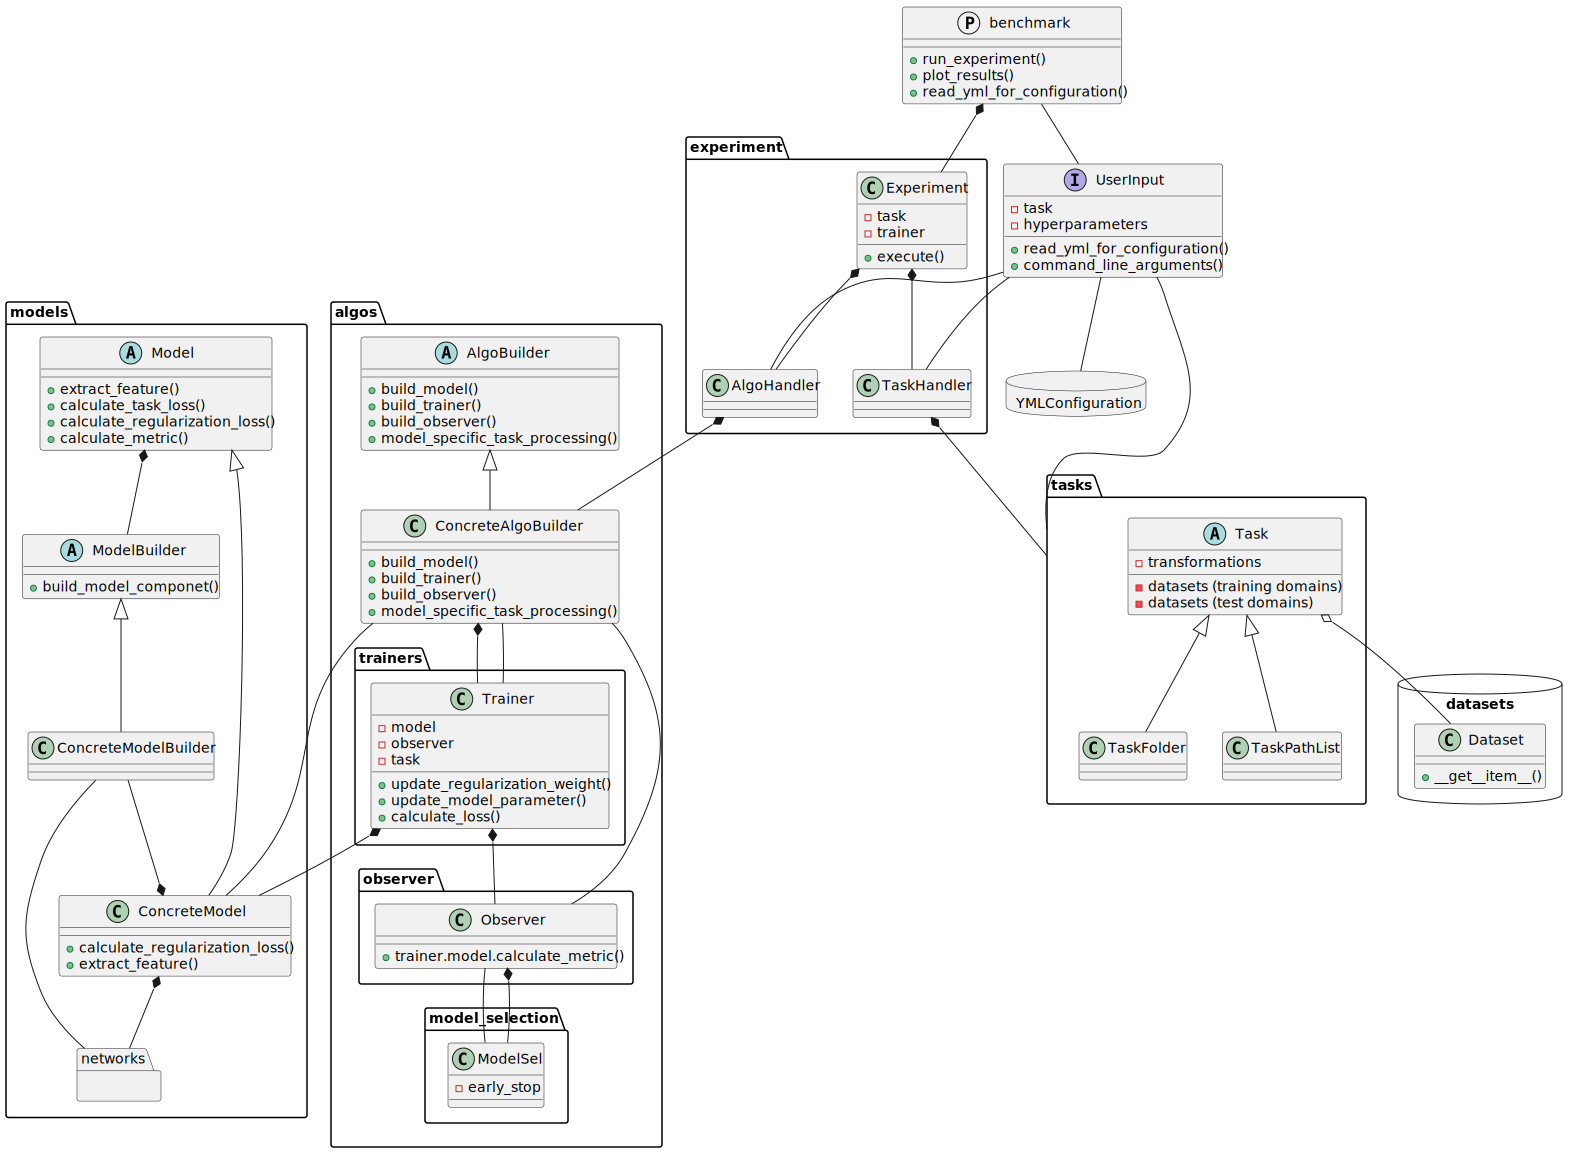
\includegraphics{../docs/libDG}
\caption{DomainLab design architecture~\label{fig:cdiagram}}
\end{figure}

\hypertarget{availability}{%
\section{Availability}\label{availability}}

Domainlab is open source and freely available. It is published under the
MIT License. Users can download the source code at
\url{https://github.com/marrlab/DomainLab}. Extensive documentation can
be found here at \url{https://marrlab.github.io/DomainLab}. DomainLab
can be installed using the
\href{https://python-poetry.org/}{python-poetry} or
\href{https://pypi.org/project/pip/}{pip} utilities.


\section{Contributions}\label{contributions}
XS has designed the package with software design patterns and
implemented the package's framework, algorithms, and other components.
He initiated and made significant contributions to other aspects of the
package development. AGossmann made significant contributions to the
software design and code, testing through use in independent research
projects, and helped writing the manuscript. CM initiated the project
with XS, contributed to the code style enhancement and paper description
of Domainlab, and supervised the project. PR contributed to the package
design, code quality, and paper description. SSB helped improving the
framework, find new use cases, and enhance the readability of the code.
FB contributed to the paper description and code documentation. GS added
the possibility to benchmark different algorithms using a Snakemake
pipeline and contributed minor enhancements. CF added sanity checks for
the datasets and implemented the chart generation for the graphical
evaluation of the benchmark results. AGruber tested and evaluated the
library with real-world medical datasets and pointed out important
issues and their solutions. RS added a feature to specify command line
arguments with YAML files. XZ contributed to the printing and saving of
the confusion matrix and code improvements.


% Acknowledgements should go at the end, before appendices and references

\acks{SSB has received funding from F. Hoffmann-la Roche LTD (No grant number
is applicable) and is supported by the Helmholtz Association under the
joint research school Munich School for Data Science (MUDS). PR was
supported through an Alexander von Humboldt Foundation postdoctoral
fellowship (Grant Nr. 1221006). CM has received funding from the
European Research Council (ERC) under the European Union's Horizon 2020
research and innovation programme (Grant agreement No.~866411).
}

% Manual newpage inserted to improve layout of sample file - not
% needed in general before appendices/bibliography.
\newpage
\bibliography{bib_domainlab_jmlr_mloss}

\end{document}
